%%%%%%%%%%%%%%%%%%%%%%%%%%%%%%%%%%%%%%%%%%%%%%%%%%%%%%%%%%%%%%%%%%%%%%%%%%%%%%%
\chapter{基于代码依赖与检索增强生成的代码变更影响分析}

\section{引言}

% 在软件系统的开发周期中,随着整体架构的日益复杂以及规模逐渐扩大,程序员在进行功能迭代、Bug修复等任务时,往往会面临较大的挑战。尤其是在庞大的代码库中,程序员难以快速且高效地评估某一变更对整体系统的影响。因此,若能在工作中引入一种高效的系统或算法来自动化地分析代码变更所带来的潜在影响,将极大地提升程序维护人员的工作效率。这不仅有助于减少潜在漏洞的发生,也能够确保系统在不断演进的过程中保持高质量和稳定性。由此可见,代码变更影响分析成为了软件开发中一个亟待关注的关键问题,值得深入研究与探讨。

由于代码预训练模型优秀的泛化能力和知识迁移能力,第二章中基于代码预训练模型的变更影响分析方法相较于基于方法间关系的方法具有更优秀的性能。但是由于其计算效率问题,导致其在实际使用时较为耗时。除此之外,由于该方法仅靠两两方法体的代码进行变更影响关系的检测,因此方法代码中无法反映的间接依赖信息在检测时缺失了,导致其在间接依赖的影响关系判断上表现不好。

检索增强生成(Retrieval Augmented Generation,RAG)技术由Lewis 等人\cite{2020Retrieval}于 2020 年提出,是一种将信息检索与生成式模型(如 GPT 等)相结合的技术,它可以在文本生成过程中有效利用外部知识库或数据库中的信息,以提高生成结果的准确性和上下文相关性。RAG工作流程可以概括为两步,检索和生成。检索过程中根据输入问询(query),从外部知识库(如文档库、网页、数据库)中检索与输入相关的上下文或片段,生成阶段将检索到的信息与用户的输入结合起来,作为生成模型的输入,生成模型根据检索的上下文生成答案或内容。RAG方法能有效解决端到端问答模型的效率问题和减少事实错误的发生。

为了进一步提升代码变更影响分析的效率和可用性,本章提出了一种基于代码依赖与检索增强生成的代码变更影响分析算法。本方法以代码库中的海量方法体为知识库,通过信息检索技术,生成候选方法集合,如果候选方法中有与变更方法存在间接依赖关系的方法,则根据代码依赖图提取调用路径上的中间方法,构造推理信息。利用当前大规模语言模型在各种文本领域上强大的语义理解和生成能力,准确的判断候选集合中的变更影响关系。

在该算法中,信息检索模块能够显著降低计算时间,确保在大规模代码库中快速定位相关代码,通过提供调用路径的中间方法,保证模型判断时的代码逻辑的完整性,而大语言模型部分则保证了变更影响关系分析结果的高准确性。此外,通过动态调整候选集合的大小,可以有效平衡算法的运行速度与分析效果,从而使得整个系统既高效又可靠,能够在实践中为程序维护和优化提供有力支持。

\section{研究动机}

上一章节所提出的基于代码预训练模型的变更影响分析方法,尽管在测试基准方面取得了当前最优的效果,然而,其仍然存在两个较为显著的问题,即计算效率问题和间接依赖的语义缺失问题。

\textbf{计算效率问题:}每当需要针对代码库中的一个变更点展开变更影响分析时,都必须将变更方法体与整个代码库的其他方法体组对,然后输入模型进行检测。对于规模较大的项目代码而言,这种方法所带来的计算延迟会严重影响其可用性,几乎使其无法正常使用。

针对该问题,可以考虑将对方法体的编码与变更关系的分析两个阶段进行解耦。在初始化阶段,运用嵌入模型对代码库的全部方法体进行编码并存储。当需要对某个变更点进行分析时,仅需通过向量相似度计算筛选出少量候选方法,利用大语言模型优越的语义理解能力进行其变更影响关系的判断。

\textbf{间接依赖的语义缺失问题:}由于基于代码预训练模型的算法仅依据两个方法体的代码来判断变更影响关系,因此当两个方法体之间存在间接依赖时,如果不提供中间方法的调用逻辑,相关信息便会缺失,这将导致模型无法合理推断方法之间的变更影响关系。在这种情况下,只有资深工程师凭借对方法功能的了解,结合丰富的经验才能够完成判断,但即便如此,也很难保证判断的正确性。

针对该问题,可以考虑在判断间接依赖的方法体之间的变更影响关系时,提供其调用路径中的中间方法,补全缺失信息,以便为模型提供支持,实现准确的判断。

因此,本章提出了基于代码依赖与检索增强生成的代码变更影响分析技术。该技术借助检索方式和代码依赖图,分别解决计算效率问题以及间接依赖所带来的语义缺失问题,从而提升变更影响分析在实际应用中的效果。


\section{基于代码依赖与检索增强生成的变更影响分析方法}


\subsection{整体流程设计}

为了解决第二章中基于代码预训练模型方法的计算效率问题与间接依赖语义缺失问题,本章提出了基于代码依赖与检索增强生成的变更影响分析方法。图\ref{2_基于代码依赖与检索增强生成的变更影响分析方法框架}中展示了本章方法的研究框架。本章的方法主要流程分为三个阶段:

\begin{enumerate}

    \item \textit{数据构建;}主要需要构建两个部分的数据:(1)代码依赖图。构建完整代码库以方法为粒度的代码依赖图,以支持后续间接调用的检测与查询。(2)嵌入模型训练需要的三元组语料。将完整代码库按照方法的粒度进行切分并作为知识库;以上一章节的依赖闭包、克隆检测、共现关系挖掘三种方法检测出的变更影响关系为原始数据,基于大预言模型与代码依赖图进行数据清洗,构建准确的变更影响关系方法三元组(查询,正例,负例),用于训练嵌入模型,使嵌入模型专精于检测变更影响关系这一垂直领域。

    \item \textit{检索模块;}在三元组语料上训练嵌入模型,并使用嵌入模型对知识库进行预编码。在测试时仅需对查询方法进行编码,并与知识库中的向量计算相似度,找出相似度最高的前$k$个(top-$k$)作为候选方法。
    
    \item \textit{增强生成;}构建由变更点方法,候选方法集合,调用路径的中间方法(如有)组合成的提示,使用大语言模型对候选方法进行判断,得到最终的有变更影响关系的方法。
    
\end{enumerate}

\begin{figure}[htbp]
\centering
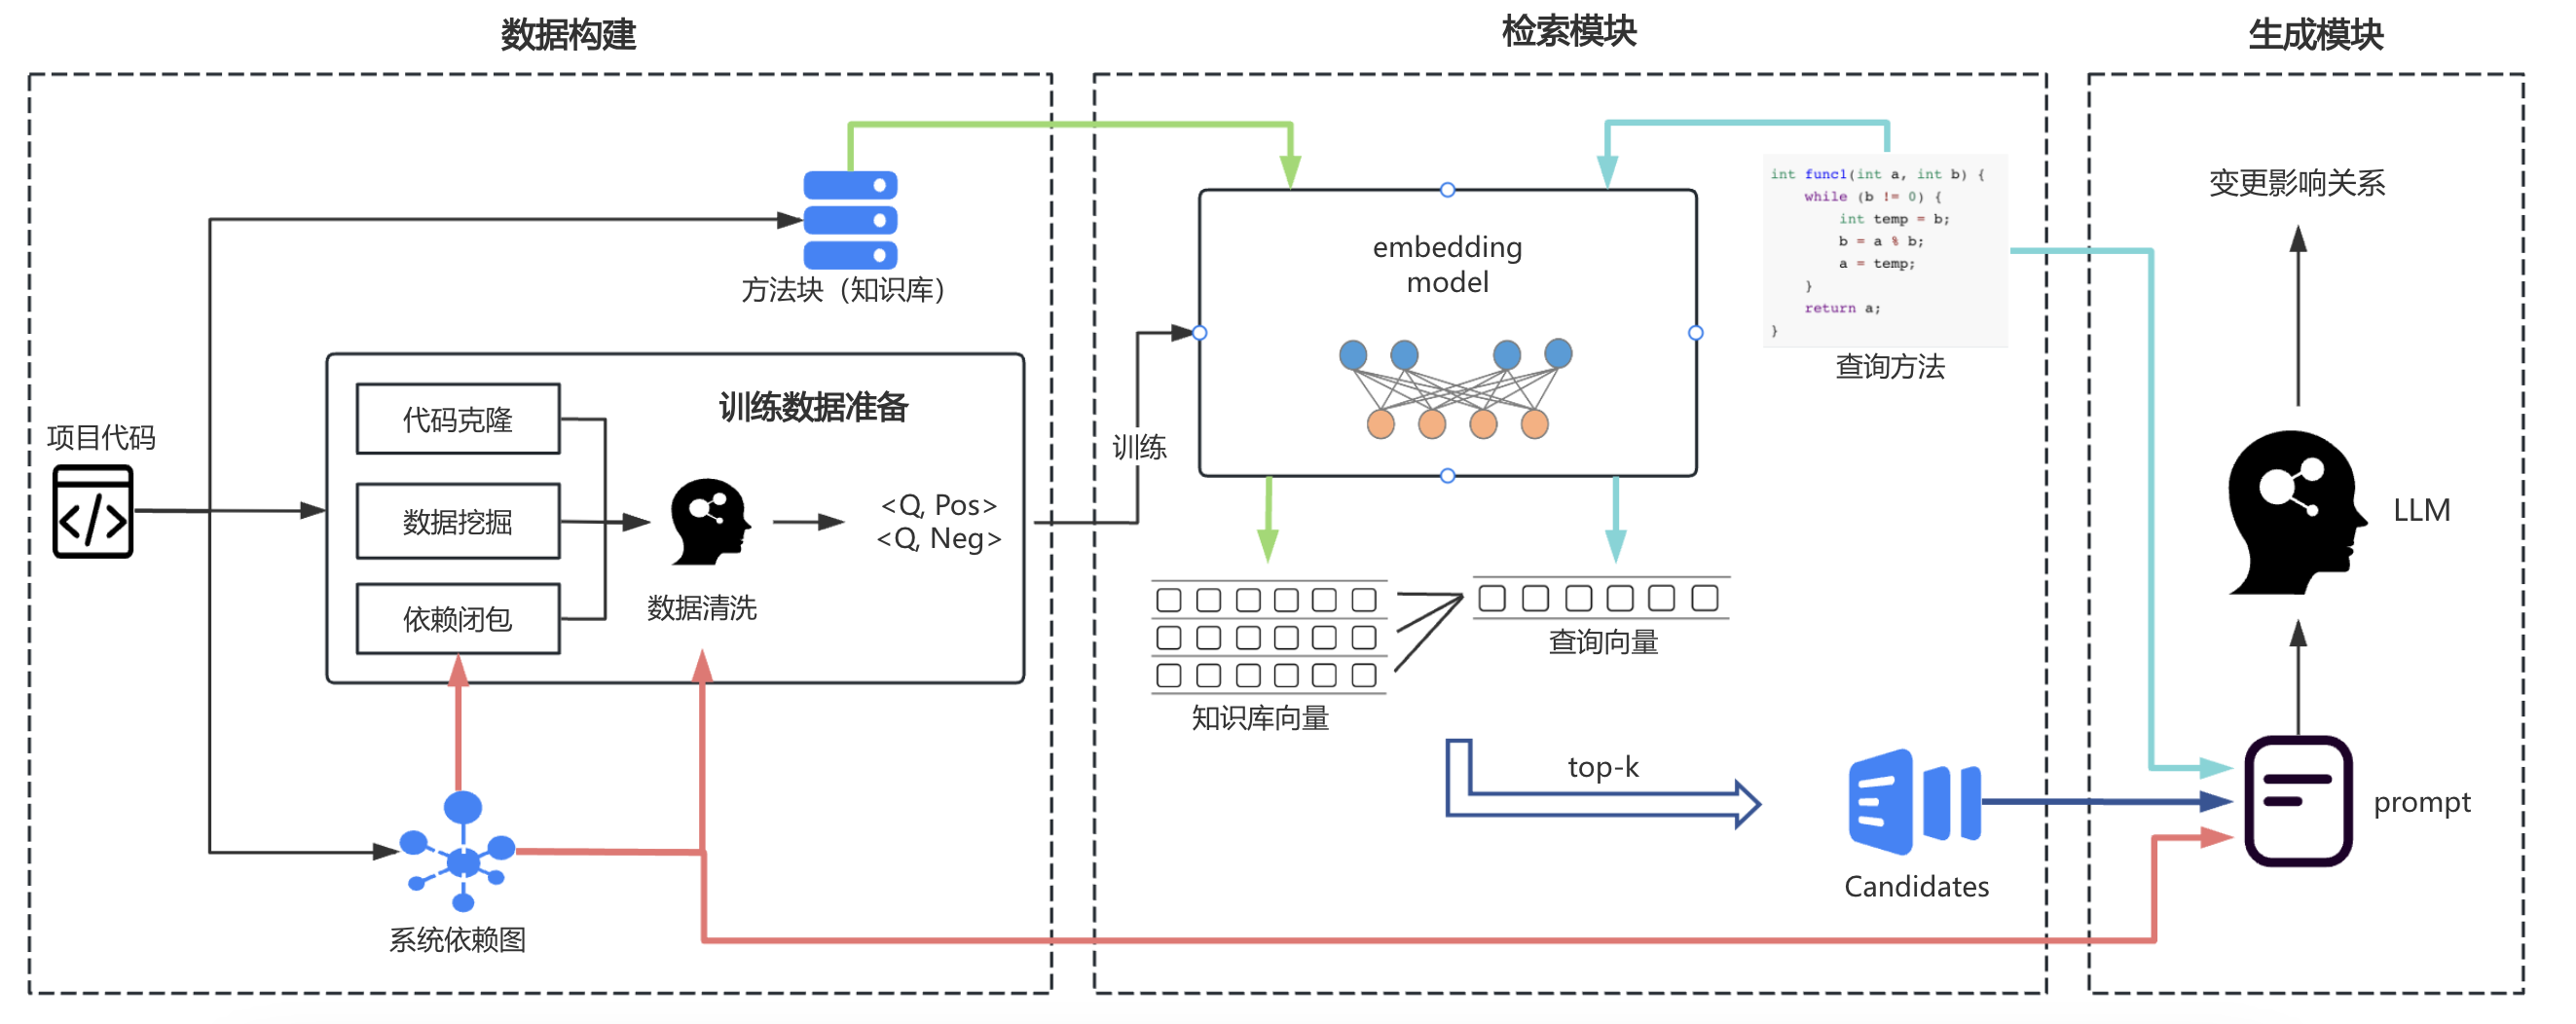
\includegraphics[width = 1\textwidth]{RAG架构.jpg}
\caption{基于代码依赖与检索增强生成的变更影响分析方法框架}
\label{2_基于代码依赖与检索增强生成的变更影响分析方法框架}
\end{figure}


\subsection{数据构建}


\paragraph{1. 代码依赖图构建} 对被分析的整个代码库按照方法的粒度进行切分,根据章节\ref{1_代码依赖图}所述,构建以方法体为顶点,以调用关系为边的代码依赖图。

\paragraph{2. 嵌入模型训练数据构建} 为了让检索模块对变更影响关系的召回率足够高,需要对嵌入模型进行训练,使具有变更影响关系的方法在向量空间中更接近,因此需要构建嵌入模型的训练数据。我们以上一章节的依赖闭包、克隆检测、共现关系挖掘三种方法检测出的变更影响关系为原始数据,使用大语言模型进行数据清洗,以得到足够准确的正例对,并对正例对中任选其一在项目中随机采样得到对应的负例,得到训练嵌入模型所需的$<Query,Pos,Neg>$三元组数据。

假设上一章节的依赖闭包、克隆检测、共现关系挖掘三种方法检测出的变更影响关系对集合为$S_{raw}$,其中$<Code_i,Code_j>\in S_{raw}$,参考上一章节的实验部分可知,$S_{raw}$中存在部分误报关系,如果不加处理,会严重影响检索模块的性能。

在对$S_{raw}$进行数据清洗时,由于在前文中提到,深度学习方法对于间接依赖导致的变更影响关系检测效果较差,正是由于方法间的间接调用信息存在缺失导致的。由此我们考虑结合依赖路径进行数据清洗。对于每一对$<Code_i,Code_j>$,数据清洗流程如下:


(1)判断依赖可达性;根据代码依赖图判断两个方法体之间是否存在调用关系,如果是直接调用,则无需处理;如果是间接调用,则需要补充调用路径的中间方法为$<Code_i,Code_{mid_1},Code_{mid_2},Code_j>$。

(2)基于大模型进行变更影响关系判断;利用代码能力与语言理解能力出色的大预言模型,为原始数据$S_{raw}$中的每一组数据构建如下图\ref{2_数据清洗prompt}的提示,进行变更影响关系的判断,剔除大模型认为没有变更影响关系的数据,剩下的数据整合为$S_{filtrate}$,其中$<Code_i,Code_j>\in S_{filtrate}$。

\begin{figure}[htbp]
\centering
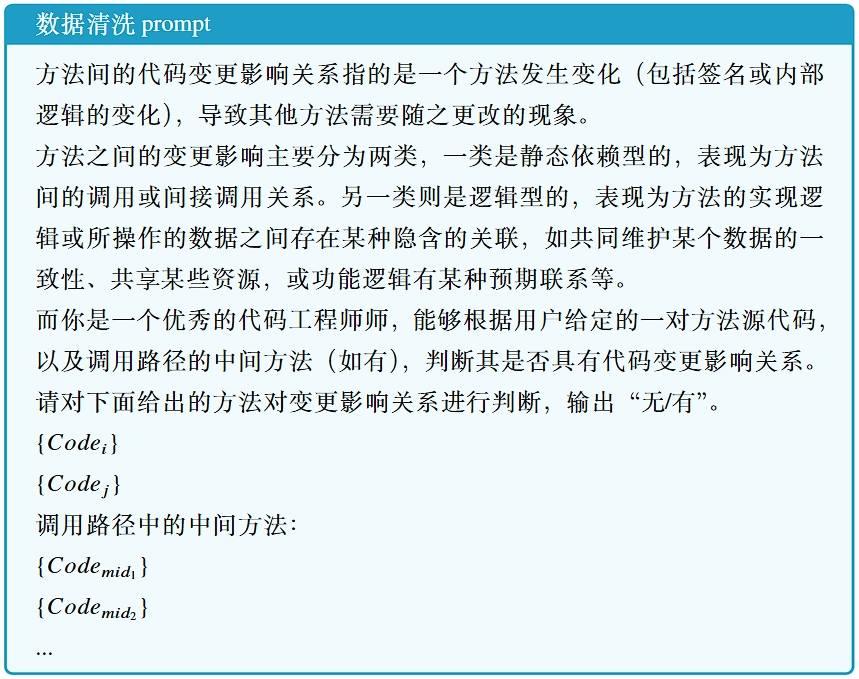
\includegraphics[width = 0.85\textwidth]{figures/2_数据清洗prompt.png}
\caption{数据清洗所使用的的Prompt}
\label{2_数据清洗prompt}
\end{figure}


接下来为$S_{filtrate}$中的数据采样负例,对于每组数据$<Code_i,Code_j>$,随机挑选其中一个方法作为查询$Code_{query}$,另一方法作为正例$Code_{pos}$统计$S_{filtrate}$中出现的$Code_{query}$的正例集合 $\{Code_{pos},Code_k,Code_e,Code_k,\}$,从代码库中除正例集合之外的方法中随机采样方法作为负例$Code_{neg}$,将构建好的三元组数据$<Code_{query},Code_{pos},Code_{neg}>\in S$作为嵌入模型的训练数据,我们之后简写为$<Query,Pos,Neg>$。

\subsection{检索模块}

检索模块主要分为离线和在线两个阶段。

离线阶段的主要任务是完成嵌入模型的训练,并对知识库中每个方法体进行嵌入。具体而言,嵌入模型通过对代码库中的每个方法进行编码,将其转换为具有语义信息的稠密向量表示。这些嵌入向量随后被存储在知识库中,为后续的检索任务提供基础。

在线阶段则针对每个查询进行实时处理。首先,通过嵌入模型将查询内容转化为稠密向量表示。然后,基于该查询向量与知识库中已嵌入方法体的向量进行相似度计算。最后,按照相似度排名从知识库中选出Topk个与查询向量相似度最高的方法体,作为疑似具有变更影响关系的候选方法。

\paragraph{1. 嵌入模型的训练}

嵌入模型通常用于将文本数据这种长度不一、非对齐的形式转换为固定长度的稠密向量表示。具体来说,对于一段文本数据$text={t_1, t_2, ..., t_n}$。对于训练数据中的三元组数据的嵌入$<E_{Query},E_{Pos},E_{Neg}>$,因为其用途一般是为了完成高效的检索,因此训练目标与使用场景相对应,希望达到的效果是将$E_{Query}$与$E_{Pos}$的相似度尽可能地提高,将$E_{Query}$与$E_{Neg}$的相似度尽可能地降低。在实际训练是经常使用对比损失函数 InfoNCE Loss 进行训练:

为了实现这一目标,通常采用对比损失函数(Contrastive Loss),其中InfoNCE Loss是一种常用的选择。其定义为:

\begin{equation}
    L_{InfoNCE} = -\log\frac{\exp(sim(E_{Query}, E_{Pos}) / \tau)}{\exp(sim(E_{Query}, E_{Pos}) / \tau)+\exp(sim(E_{Query}, E_{Neg}) / \tau)}
\end{equation}

其中,$\tau$为温度因子,用于控制相似度的平滑程度。通过最小化$L_{InfoNCE}$来优化嵌入模型,从而提升查询向量与正样本之间的相似度,同时减少与负样本之间的相似度。

为了与后续在线相似度计算的工程实现相匹配,本文在相似度度量上选择了欧式距离(L2距离):

\begin{align}
sim(A,B)&=-L2(A, B)  = -\sqrt{\sum_{i=1}^{n} (y_i - x_i)^2} \\
A &= (x_1, x_2, \dots, x_n) \\
B &= (y_1, y_2, \dots, y_n)
\end{align}

\paragraph{2. 知识库的构建}

在训练出嵌入模型后,为了在实际应用中提升推理速度,必须基于完整的代码库构建一个知识库。这一过程旨在将代码库中的每个方法体转换为具有语义信息的稠密向量表示,从而便于在推理过程中高效地进行检索。具体而言,使用前一章节中训练得到的嵌入模型对代码库中的每个方法体$Code_i$进行编码,得到对应的向量表示$E_{Code_i}=Embedding\_model(Code_i)$,其中每个$E_{Code_i}$是一个包含该方法语义信息的稠密向量。经过编码后,所有方法体的向量集合为$\mathbf{E}={E_{code_1}, E_{code_2}, ..., E_{code_n}}$,其中$n$表示代码库中方法体的总数。

为了提高知识库检索的效率,本研究采用了FAISS(Facebook AI Similarity Search)作为稠密向量的检索工具。FAISS是一种高效的向量检索框架,能够对大规模向量数据进行索引并支持快速检索。通过构建向量索引,FAISS能够显著提高在大规模数据库中进行相似度搜索的速度。FAISS支持多种类型的索引结构,包括平坦索引、倒排文件索引和层次化导航图等,这些索引结构能够根据数据的规模、向量维度及存储需求,灵活应对不同查询速度和精度的需求。

鉴于本文的研究对象是软件项目代码,且分析粒度为方法级别,代码库中的方法数量通常较少,最多只有几千个方法。与处理文档类问答生成任务中涉及的大规模数据集不同,本文的代码库规模相对较小。因此,在构建索引时,本文选择了较为简单的平坦索引结构对方法向量进行检索。

\paragraph{3. 查询的嵌入}

在实际使用中,到达一个新的查询$Query$,使用上文经过训练的嵌入模型进行嵌入$E_{Query}=Embedding\_model(Query)$;

\paragraph{4. 知识库的检索}

在获得查询的嵌入表示$E_{Query}$之后,便可以利用FAISS对知识库中的向量进行检索,选择与查询向量$E_{Query}$在L2距离上最为接近的$k$个向量。通过这些相似度最高的$k$个向量的索引,可以找到对应的源码方法,并将其作为候选方法返回。具体来说,$top\ k$值的选择对检索结果的质量与效率有着直接影响。

当$top\ k$值设置得较高时,检索模块能够召回更多的正确关系,因此系统的查全率较高。然而,随着候选数量的增加,后续的大模型需要判断更多的候选方法,导致整个系统的处理速度可能会下降。相反,若$top\ k$值设置较低,则检索出的候选方法较少,查全率可能会较低,但系统的响应速度会相对较快。因此,$top\ k$的选择需要根据实际使用场景的需求以及模型的能力进行权衡,以达到查全率与速度之间的最佳平衡。


\subsection{生成模块}

生成模块希望利用大规模语言模型优秀的语义理解能力,对查询方法$Code_{query}$和检索出来的候选方法$\{Code_1,Code_2,...,Code_k\}$进行代码变更影响关系的判断。在判断之前需要根据代码依赖图判断查询方法与候选方法之间是否存在调用关系,如果是直接调用,则无需处理;如果是间接调用,则需要补充调用路径的中间方法为$<Code_{query},Code_{1_{mid_1}},...,Code_{1_{mid_2}},Code_1>$。接下来构建如图\ref{2_推理prompt}所示的提示使用大规模语言模型进行变更影响关系判断。

\begin{figure}[htbp]
\centering
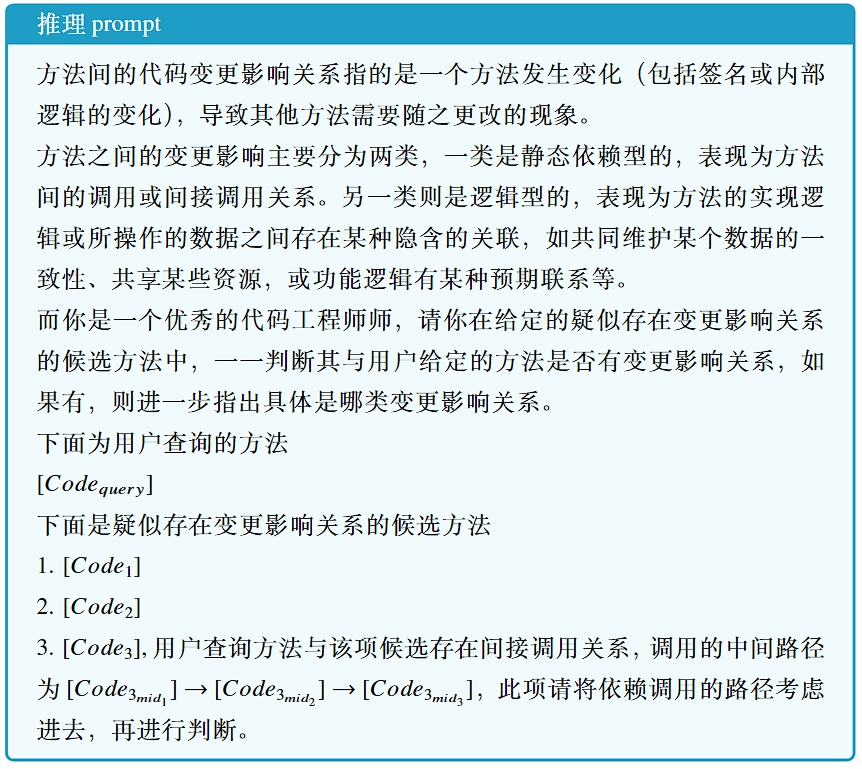
\includegraphics[width = 0.85\textwidth]{figures/2_推理prompt.png}
\caption{生成模块所使用的的Prompt}
\label{2_推理prompt}
\end{figure}


将大语言模型的回复进行解析即可得到与查询方法有变更影响分析的方法。对于有$N$个方法的项目,在实际使用时对于每个查询,需要进行$N$次相似度计算,调用$1$次大模型进行推理,如果上下文长度过长可以对候选方法分片,多次调用大模型,相比于基于代码预训练模型的方法每次需要$N$次的模型前向计算,不仅节省了大量计算时间,还提升了系统的查全率查准率,在实际应用场景中是更好的选择。


\section{实验结果与分析}

\subsection{数据集}
为了便于与前文方法进行性能对比,本章同样选择了六个具有一定规模和影响力的开源代码库作为实验对象,具体包括TheAlgorithms、antiword-0.37、jemalloc-5.3.0、libbpf-1.1、librdkafka-2.1.0和FFmpegKit-5.1.0。这些代码库的选择考虑了其广泛应用和代表性,能够较好地反映方法在实际开发环境中的效果。

鉴于本章提出了一种基于代码依赖的数据清洗方法,嵌入模型所需的训练数据经过重新清洗,以确保其质量和准确性。数据集的收集过程与\ref{1_数据集来源和数据清洗}节中的方法一致。在数据清洗过程中,所使用的模型为Doubao(API模型名:Doubao-lite-32k-240428),该模型在处理代码依赖关系和数据清洗任务方面表现出较高的精度。最终,得到的训练数据的统计信息如表\ref{1_数据集统计信息}所示,共计包含6526对数据。这些数据将用于后续方法的训练。


\begin{table}[htbp]
\caption{训练数据统计信息}
\label{1_数据集统计信息}
\vspace{0.5em}\centering\wuhao
\begin{tabular}{cccc}
\toprule
项目名称 & 三元组数量 \\
\midrule
TheAlgorithms    & 314   \\
antiword-0.37    & 257   \\
jemalloc-5.3.0   & 1023   \\
libbpf-1.1       & 835   \\
librdkafka-2.1.0 & 1524  \\
FFmpegKit-5.1.0  & 336   \\ 
总计              & 4289  \\
\bottomrule
\end{tabular}
\end{table}

\subsection{评价指标} 
评价指标同第\ref{1_评价指标}节,使用Precision,Recall和F-measure来评价模型挖掘变更影响关系的能力。

\subsection{实验设置}

\paragraph{1. 检索模块嵌入模型选择}
MTEB Leaderboard\footnote{https://huggingface.co/spaces/mteb/leaderboard} 是一个实时更新的开源嵌入模型排行榜,专门用于评估不同模型在各种任务中的嵌入能力。为了实现对知识库中代码片段的有效编码,本文从MTEB Leaderboard中选取适合本任务的嵌入模型。选择标准主要包括以下几点:(1)模型在开源嵌入能力评价基准上表现优异,这能够体现其在各类通用文本上的嵌入能力;(2)模型支持的上下文长度大于4k,考虑到代码任务通常涉及较长的上下文,较短的上下文长度可能无法有效捕捉到代码间的复杂关系;(3)模型的参数规模控制在500M以下,综合考虑计算资源和数据规模,超过500M参数规模的模型在使用上的代价较高,难以满足实际应用需求。基于这些选择标准,本文最终选定了如表\ref{2_嵌入模型参数量}所示的5个模型。这些模型在性能、上下文支持以及资源消耗方面都达到了较好的平衡,适合本研究中对代码片段进行嵌入编码的需求。
    
    \begin{table}[htbp]
    \caption{嵌入模型信息}
    \label{2_嵌入模型参数量}
    \vspace{0.5em}\centering\wuhao
    \begin{tabular}{ccc}
    \toprule
    嵌入模型 & 参数量 & 上下文长度  \\
    \midrule
    gte-large-en-v1.5 & 434M & 8192 \\
    jina-embeddings-v3 & 572M & 8192\\
    stella\_en\_400M\_v5 & 435M & 8192 \\
    KaLM-embedding-multilingual-mini-instruct-v1.5 & 494M & 131072 \\
    nomic-embed-text-v1.5 & 137M & 8192 \\
    \bottomrule
    \end{tabular}
    \end{table}
    
\paragraph{2. 嵌入模型训练设置}
在本研究的嵌入模型训练过程中,采用了对比损失函数(InfoNCE Loss)作为目标函数,以确保模型能够有效学习到不同代码片段之间的相似度关系。训练优化器选择了Adam优化器,其中超参数$\beta_1$设置为0.9,$\beta_2$设置为0.95。为提高训练效果,学习率采用余弦衰减策略,使得训练过程中学习率逐渐减小,有助于模型在接近收敛时获得更精细的更新。

Batch size固定为64,以保证每次梯度更新的稳定性。对于较大规模的模型,考虑到内存限制,采用了梯度累计(Gradient Accumulation)技术,通过多次反向传播累积梯度,从而保证了相同的批次大小。学习率初始值设置为1e-4。

在训练阶段,损失函数设置为对比损失函数InfoNCE Loss。训练优化器使用Adam,超参数$\beta_1$设置为0.9,$\beta_2$设置为0.95;学习率采用余弦衰减;Batchsize固定为64,对于规模较大的模型,使用梯度累计方法保证batchsize大小。学习率设置为1e-4。所有实验均在PyTorch框架和Transformer库上实现,确保了高效的模型训练和易于扩展的实现平台。训练过程在单个NVIDIA Tesla V100 32G GPU上进行。
    
\paragraph{3. 生成模型选择}
本章实验中生成模块使用的大模型包含两类:闭源商业模型和开源模型;其中闭源模型包括:GPT4o(API model name:gpt-4o-2024-05-13),Doubao(API model name:Doubao-lite-32k-240428),Kimi(API model name:moonshot-v1-32k);开源模型选择:Qwen2.5-Coder-3B-Instruct ,Llama-3.2-3B-Instruct


\subsection{实验结果与分析}

RQ1:检索模块性能如何,是否能有效地检索到与问询方法存在变更影响关系的方法?

RQ2:本章提出的基于代码依赖与检索增强生成的变更影响关系分析方法性能如何,相比于其他方法表现如何?

RQ3:本章提出的基于代码依赖与检索增强生成的变更影响关系分析方法是否能有效解决间接依赖信息缺失的问题?

RQ4:本章提出的基于代码依赖与检索增强生成的变更影响关系分析方法的跨项目迁移表现如何?
 

\textbf{1.针对于RQ1的实验}

检索模块的嵌入模型表现如表\ref{1_检索模块的召回率与Topk的关系可视化}所示。其中横坐标表示$topk$,即返回检索模块对知识库的相似度排序的前$k$个作为候选,纵坐标表示召回率。虚线为未经训练的嵌入模型,实现表示经过训练的嵌入模型。


\begin{figure}[htbp]
\centering
\includegraphics[width = 1\textwidth]{figures/topk召回率可视化.pdf}
\caption{检索模块的召回率与Topk的关系可视化}
\label{1_检索模块的召回率与Topk的关系可视化}
\end{figure}

可以发现经过训练的模型在本文应用场景性能更好,其中经过训练的stella\_en\_400M\_v5综合表现最佳,考虑到$topk$的大小会对推理速度和召回率产生相反的影响,综合考虑选择$topk=20$作为后续实验的设定。 

\textbf{2.针对于RQ2的实验}

关于生成模块中不同大语言模型对最终性能影响如表\ref{2_不同LLM的实验表现}所示,GPT4o是综合表现最佳的生成模块的选择,即使最小的开源模型Qwen2.5-Coder-3B-Instruct ,Llama-3.2-3B-Instruct也可以超过经过上一章节训练的CodeBERTa模型。

\begin{table}[htbp]
\caption{不同LLM的实验表现}
\label{2_不同LLM的实验表现}
\vspace{0.5em}\centering\wuhao
\begin{tabular}{cccc}
\toprule
方法 & F-measure & recall & precision  \\
\midrule
CodeBERTa & 59.5 & 55.3 & 64.4 \\
Just Retrieval & 32.6 & \textbf{78.1} & 20.6 \\
\midrule
RAG-GPT4o & \textbf{74.8} & 74.6 & \textbf{75.1} \\
RAG-Doubao & 73.4 & 73.8 & 73.1 \\
RAG-Kimi & 71.9 & 71.2 & 72.7 \\
RAG-Qwen2.5 & 65.4 & 63.5 & 67.4 \\
RAG-Llama-3.2 & 64.9 & 62.3 & 67.8 \\
\bottomrule
\end{tabular}
\end{table}


表\ref{2_变更影响实验结果}进一步对于不同类型的影响关系进行分析,可以发现相比于之前方法来讲,基于代码依赖与检索增强生成的方法在两个类型的变更影响关系检测上,均拥有更好的性能。其中依赖型关系的F-measure提升更是达到16.9\%,其中由于增添了检索模块,在两种关系的召回率方面提升显著。

\begin{table}[htbp]
\caption{变更影响实验结果}
\label{2_变更影响实验结果}
\vspace{0.5em}\centering\wuhao
\begin{tabular}{c|ccc|ccc|c}
\toprule
  & \multicolumn{3}{c|}{Dependence-Based} & \multicolumn{3}{c|}{Logic-Based} & Overall \\
\midrule
方法 & F-measure & recall & precision & F-measure & recall & precision  
 & F-measure\\
\midrule
依赖闭包 &  44.8 & 100 & 28.9 & - & - & - & 36.8 \\
克隆检测 &  - & - & - & 31.8 & 19.1 & 95.7 & 3.8\\
共现关系挖掘 &  56.0 & 44.6 & 75.4 & 57.0 & 47.3 & 71.8 & 52.8\\
CodeBERTa  &   61.9 & 56.6 & 68.3 & 71.7 & 73.9 & 69.7 &59.5\\
Just Retrieval   & 34.5 & 82.3 & 21.8 & 36.6 & 88.5 & 23.1 & 32.6\\
RAG & \textbf{78.8} & 78.4 & 79.2 & \textbf{85.4} & 85.9 & 84.9 & \textbf{74.8}\\
\bottomrule
\end{tabular}
\end{table}

\textbf{3.针对于RQ3的实验}

本实验探讨在提示中加入调用路径的中间方法对间接依赖的检测效果的影响。选取测试集中的间接依赖型的变更影响分析子集进行实验,结果如图\ref{2_消融实验}所示。根据结果可以看出在提示中加入调用路径的中间方法对于基于RAG的方法在提升非常显著。

\begin{table}[htbp]
\caption{加入调用路径的中间方法对间接依赖的检测效果的影响}
\label{2_消融实验}
\vspace{0.5em}\centering\wuhao
\begin{tabular}{cccc }
\toprule
  & \multicolumn{3}{c}{Indirect-Dependence-Based}  \\
\midrule
方法 & F-measure & recall & precision \\  
\midrule
CodeBERTa  &  10.7 & 15.1 & 8.3 \\
\midrule
RAG  & 72.6 & 73.5 & 71.7 \\
RAG without 依赖路径  & 14.2 & 12.1 & 17.1 \\
\bottomrule
\end{tabular}
\end{table}


\textbf{4.针对于RQ4的实验}

本实验探讨所提出方法在跨项目的迁移能力,数据集划分同上一章节一样,分为四个分布内代码库和两个分布外代码库。实验结果如表\ref{2_跨项目迁移能力分析}所示。上一章节的基于代码预训练模型的方法,跨项目时性能下降在28.9\% 到 31.7\%之间。本章节的检索模块以及整个RAG系统在跨项目时性能下降仅在 9.2\% 到 11.4\%。


\begin{table}[htbp]
\caption{跨项目迁移能力分析}
\label{2_跨项目迁移能力分析}
\vspace{0.5em}\centering\wuhao
\begin{tabular}{c|cccc|cc}
\toprule
方法& TheAlgorithms & antiword & librdkafka & FFmpegKit & jemalloc & libbpf\\
\midrule
train on 6 datasets:\\
\midrule
CodeBERTa  &  60.23 & 59.64 & 60.18 & 57.87 & 60.99 & 58.22 \\
Just Retrieval   & 32.4 & 32.91 & 31.81 & 36.57 & 33.78 & 35.07  \\
RAG & 76.0 & 78.45 & 76.46 & 77.66 & 79.04 & 76.29  \\
\midrule
train on 4 datasets:\\
\midrule
CodeBERTa  &  62.28 & 65.24 & 63.45 & 62.19 & 41.92$^*$ & 40.8$^*$\\
Just Retrieval   & 33.33 & 34.2 & 34.77 & 36.89 & 29.74$^*$ & 31.09$^*$ \\
RAG & 78.24 & 79.21 & 78.59 & 77.98 & 71.08$^*$ & 69.66$^*$ \\
\bottomrule
\end{tabular}
\end{table}
 

\section{本章小结}

本章提出了基于代码依赖与检索增强生成的代码变更影响分析方法,通过结合依赖路径提升了方法在间接依赖影响上的检测性能,并通过训练检索模块,大幅提升了测试集上的召回率,最后整个系统的综合表现得到了大幅提升。并且通过实验验证了依赖路径加入的有效性。最后在跨项目迁移能力的实验中,基于代码依赖与检索增强生成的代码变更影响分析方法的迁移能力表现优秀,进一步证明了本章所提出的方法的有效性。

%%%%%%%%%%%%%%%%%%%%%%%%%%%%%%%%%%%%%%%%%%%%%%%%%%%%%%%%%%%%%%%%%%%%%%%%%%%%%%%